\subsection{L-TAE}
The increasing accessibility and precision of Earth observation satellite data offers considerable opportunities for industrial and state actors alike. This calls however for efficient methods able to process time-series on a global scale. Building on recent work employing multi-headed self-attention mechanisms to classify remote sensing time sequences, we propose a modification of the Temporal Attention Encoder. In our network, the channels of the temporal inputs are distributed among several compact attention heads operating in parallel. Each head extracts highly-specialized temporal features which are in turn concatenated into a single representation. Our approach outperforms other state-of-the-art time series classification algorithms on an open-access satellite image dataset, while using significantly fewer parameters and with a reduced computational complexity.

\subsubsection{Attention Encoder}

\subsubsection{Data preparation}
- splits\\
- dates\\

\subsubsection{Model}

\begin{figure}[!htbp]
  \centering
  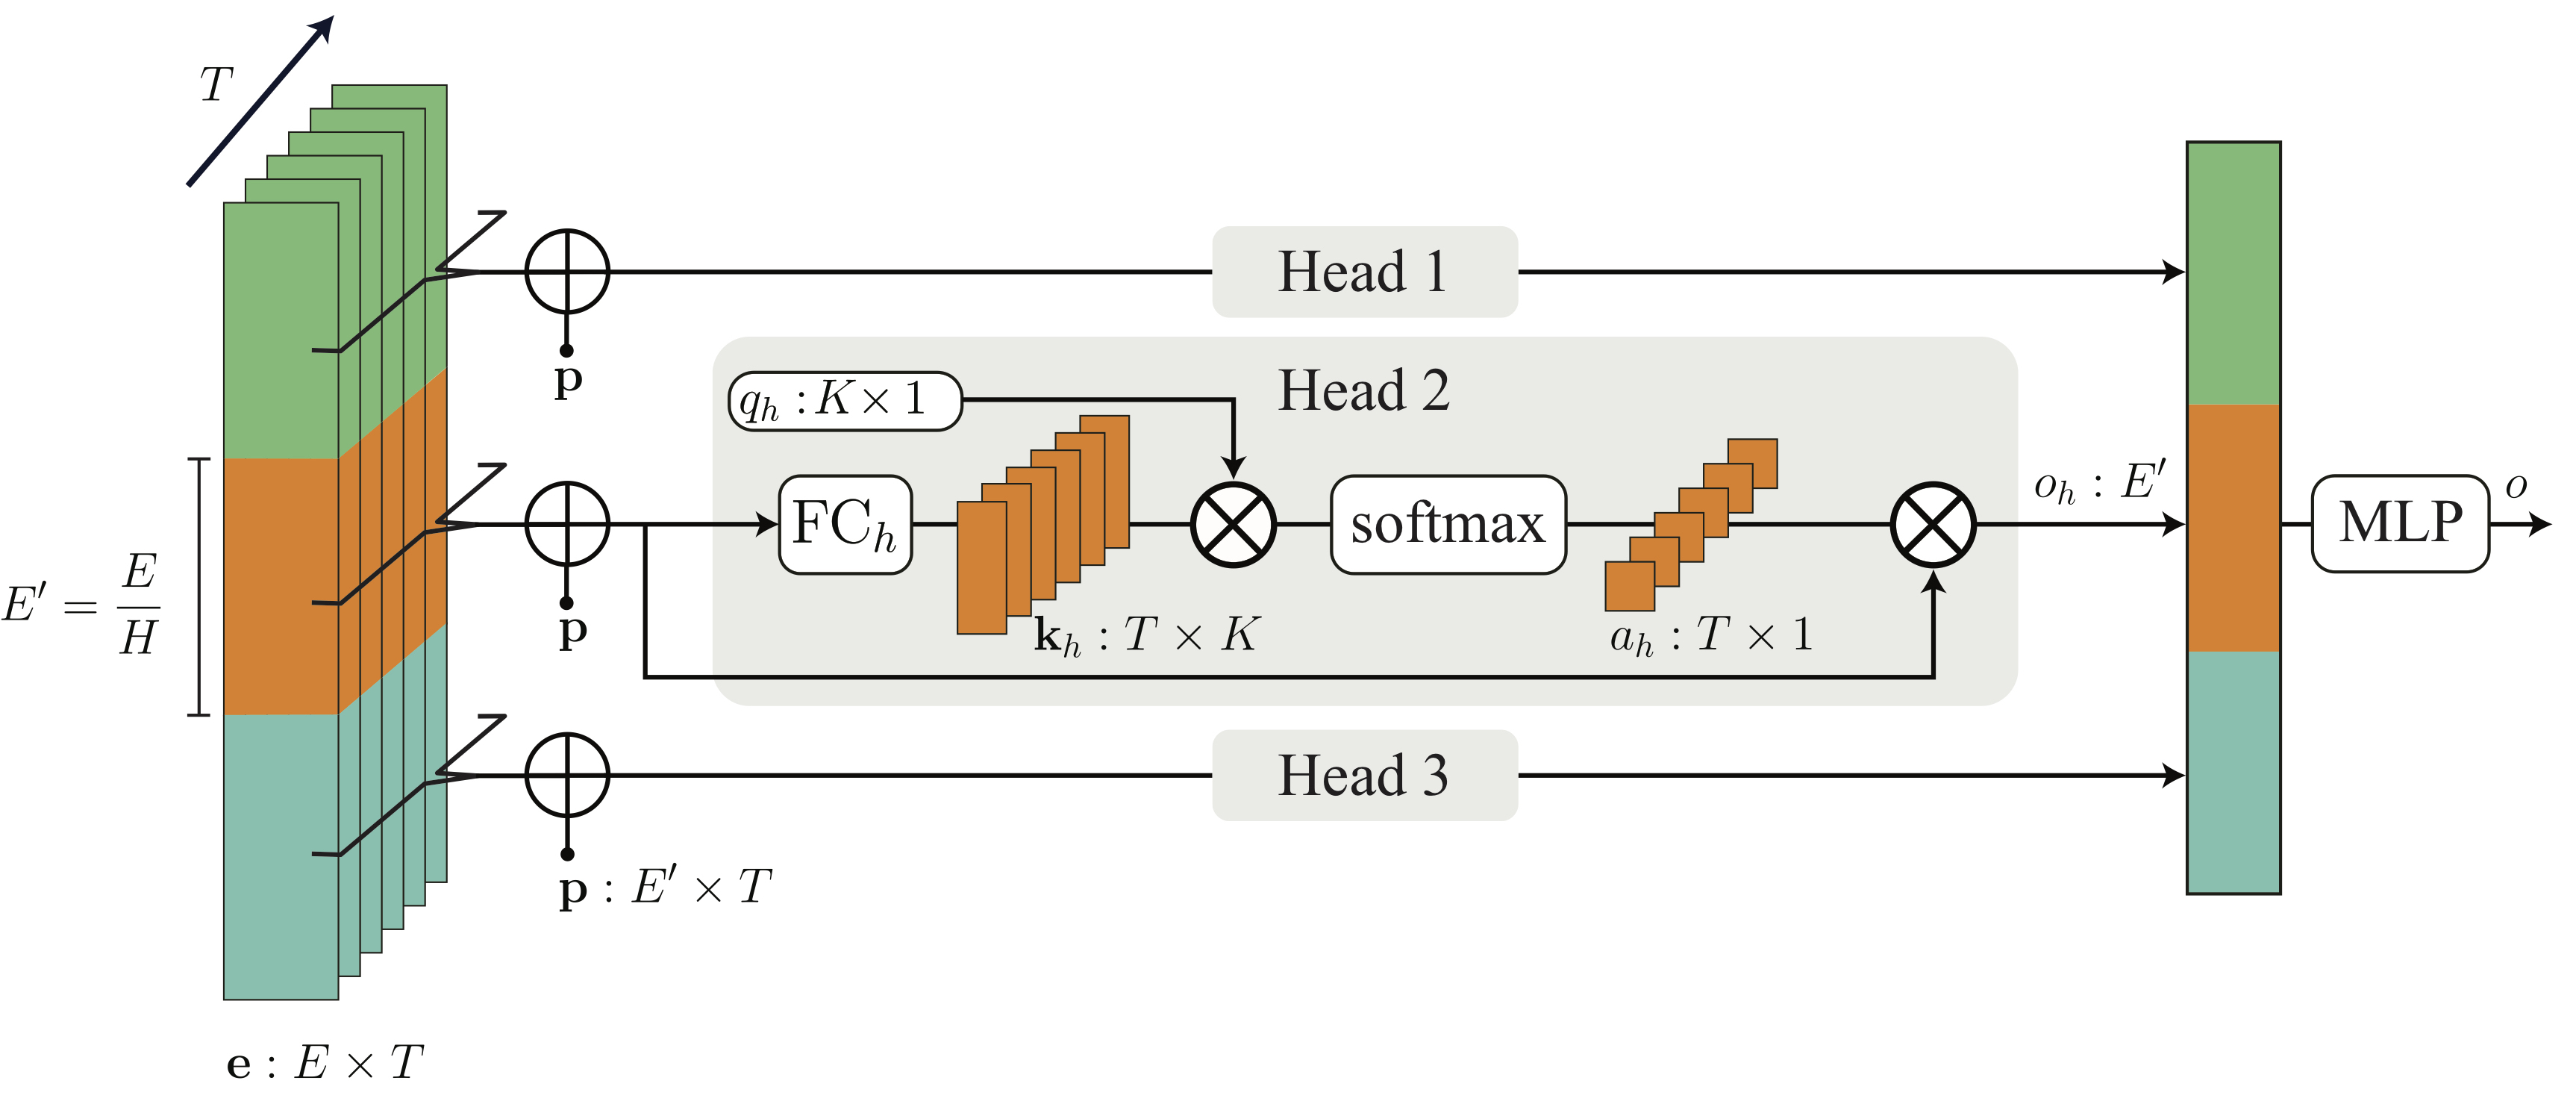
\includegraphics[width=1\textwidth]{LTAE}
  \caption{Light Temporal Attention Encoder  (L-TAE) architecture \cite{LTAE}}
  \label{tab:LTAErchitecture}
\end{figure}

- pytorch implementation\\
- PixelSetEncoder\\
- DenseEncoder

- imputation vs no imputation

- tanh

\begin{table}[ht]
  \centering
  \begin{tabular}{l p{12cm}}   
     Param & Description \\[0.2cm] 
     \hline \\[-0.2cm]  
     E & size of the embeddings ($E$), if input vectors are of a different size, a linear layer is used to project them d\_model-dimensional space \\
     H & Number of attention heads  \\
     K & Dimension of the key and query vectors  \\
     MLP & Number of neurons in the layers of MLP \\
  \end{tabular}
  \caption{Params of L-TAE model}
  \label{tab:LTAEconfig}
\end{table} 

\subsubsection{Experimental results}

\begin{table}[ht]
  \centering
  \begin{tabular}{cccclrr} 
     Params & E & H & K & MLP & No imputation & Pre imputation\\[0.2cm] 
     \hline \\[-0.2cm] 
     43k & 	128 & 	8 & 	8 & 	128 & 	$93.37 \pm 1.65$ & 	$93.08 \pm 1.16$\\ 
     68k & 	128 & 	16 & 	8 & 	128 - 128 & 	$93.43 \pm 1.37$ & 	$93.39 \pm 1.16$\\ 
     123k & 	256 & 	16 & 	8 & 	256 - 128 & 	$93.15 \pm 1.72$ & 	$93.44 \pm 1.22$\\ 
     299k & 	512 & 	32 & 	8 & 	512 - 128 & 	$\mathbf{93.65 \pm 1.30}$ & 	$93.40 \pm 1.16$\\ 
     749k & 	1024 & 	32 & 	8 & 	1024 - 256 - 128 & 	$92.91 \pm 1.90$ & 	$\mathbf{93.58 \pm 1.29}$\\ 
  \end{tabular}
  \caption{Results of the L-TAE model with different parameters}
  \label{tab:LTAEresults}
\end{table}